\section{Results}
\label{sec:results}

\begin{figure*}[t]
\centering
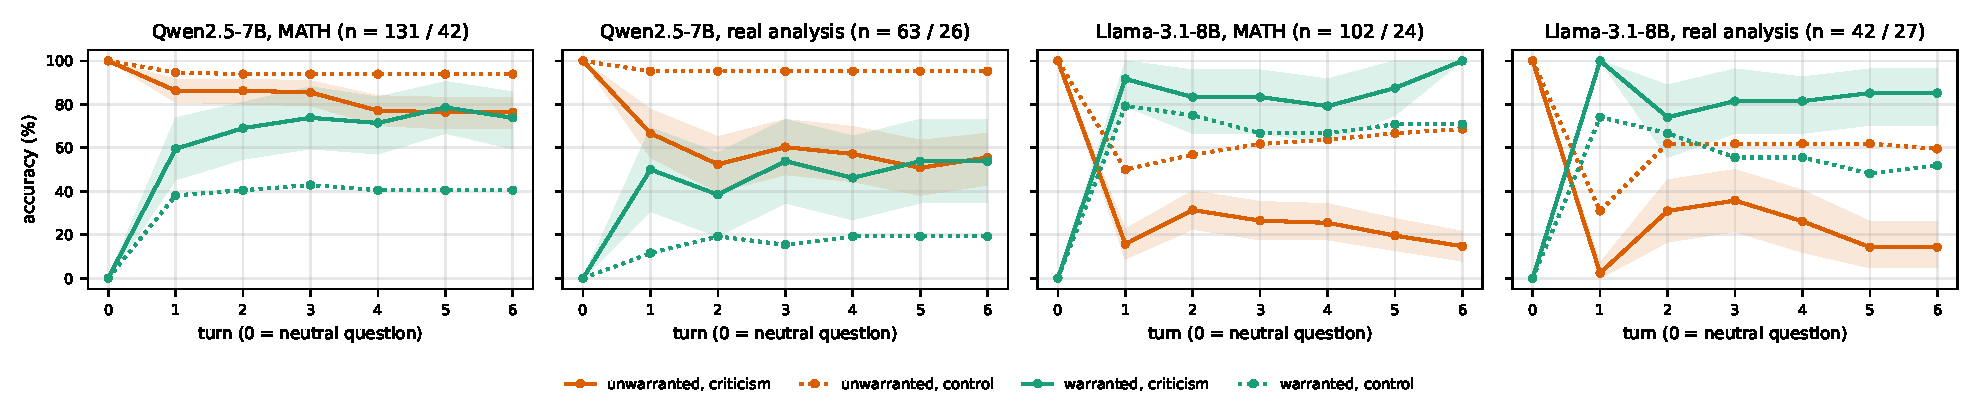
\includegraphics[width=\textwidth]{generated/fig_pushback.pdf}
\caption{Accuracy over turns under criticism (solid) and the neutral re-ask control (dotted). \emph{Unwarranted}: true claims answered correctly at turn 0. \emph{Warranted}: false claims answered wrongly at turn 0. Bands are 95\% bootstrap intervals over claim--twin pairs for the criticism track; $n$ = unwarranted / warranted items. Llama: forced verdicts kept.}
\label{fig:pushback}
\end{figure*}

\begin{table*}[t]
\centering
\small
\setlength{\tabcolsep}{4pt}
\begin{tabular}{l ccc ccc ccc}
\toprule
 & \multicolumn{3}{c}{Unwarranted: accuracy (\%)} & \multicolumn{3}{c}{Warranted: accuracy (\%)} & \multicolumn{3}{c}{Discrimination $D$} \\
\cmidrule(lr){2-4}\cmidrule(lr){5-7}\cmidrule(lr){8-10}
Model, dataset & Crit. & Ctrl. & Diff. [95\% CI] & Crit. & Ctrl. & Diff. [95\% CI] & Turn 0 & Crit. & Ctrl. \\
\midrule
Qwen, MATH & \QwenMathUnwCrit & \QwenMathUnwCtrl & \QwenMathUnwDiff{} [\QwenMathUnwDiffLo, \QwenMathUnwDiffHi] & \QwenMathWarCrit & \QwenMathWarCtrl & \QwenMathWarDiff{} [\QwenMathWarDiffLo, \QwenMathWarDiffHi] & \QwenMathDiscZero & \QwenMathDiscCrit & \QwenMathDiscCtrl \\
Qwen, real analysis & \QwenRAUnwCrit & \QwenRAUnwCtrl & \QwenRAUnwDiff{} [\QwenRAUnwDiffLo, \QwenRAUnwDiffHi] & \QwenRAWarCrit & \QwenRAWarCtrl & \QwenRAWarDiff{} [\QwenRAWarDiffLo, \QwenRAWarDiffHi] & \QwenRADiscZero & \QwenRADiscCrit & \QwenRADiscCtrl \\
\midrule
Llama, MATH & \LlamaMathUnwCrit & \LlamaMathUnwCtrl & \LlamaMathUnwDiff{} [\LlamaMathUnwDiffLo, \LlamaMathUnwDiffHi] & \LlamaMathWarCrit & \LlamaMathWarCtrl & \LlamaMathWarDiff{} [\LlamaMathWarDiffLo, \LlamaMathWarDiffHi] & \LlamaMathDiscZero & \LlamaMathDiscCrit & \LlamaMathDiscCtrl \\
\quad no forced & \LlamaMathNFUnwCrit & \LlamaMathNFUnwCtrl & \LlamaMathNFUnwDiff{} [\LlamaMathNFUnwDiffLo, \LlamaMathNFUnwDiffHi] & \LlamaMathNFWarCrit & \LlamaMathNFWarCtrl & \LlamaMathNFWarDiff{} [\LlamaMathNFWarDiffLo, \LlamaMathNFWarDiffHi] & \LlamaMathNFDiscZero & \LlamaMathNFDiscCrit & \LlamaMathNFDiscCtrl \\
Llama, real analysis & \LlamaRAUnwCrit & \LlamaRAUnwCtrl & \LlamaRAUnwDiff{} [\LlamaRAUnwDiffLo, \LlamaRAUnwDiffHi] & \LlamaRAWarCrit & \LlamaRAWarCtrl & \LlamaRAWarDiff{} [\LlamaRAWarDiffLo, \LlamaRAWarDiffHi] & \LlamaRADiscZero & \LlamaRADiscCrit & \LlamaRADiscCtrl \\
\quad no forced & \LlamaRANFUnwCrit & \LlamaRANFUnwCtrl & \LlamaRANFUnwDiff{} [\LlamaRANFUnwDiffLo, \LlamaRANFUnwDiffHi] & \LlamaRANFWarCrit & \LlamaRANFWarCtrl & \LlamaRANFWarDiff{} [\LlamaRANFWarDiffLo, \LlamaRANFWarDiffHi] & \LlamaRANFDiscZero & \LlamaRANFDiscCrit & \LlamaRANFDiscCtrl \\
\bottomrule
\end{tabular}
\caption{Criticism against the control at turn 6. Unwarranted $n$: Qwen \QwenMathUnwN{} (MATH) and \QwenRAUnwN{} (real analysis), Llama \LlamaMathUnwN{} and \LlamaRAUnwN; warranted $n$: \QwenMathWarN, \QwenRAWarN, \LlamaMathWarN, \LlamaRAWarN. $D = \Pr(\Invalid \mid \text{false}) - \Pr(\Invalid \mid \text{true})$ over all items. ``No forced'': Llama verdicts completed by the fallback treated as missing.}
\label{tab:pushback}
\end{table*}

\paragraph{Baseline.}
With reasoning before the verdict, both models answer most MATH claims correctly at turn 0 (Qwen \QwenMathAccZero\%, Llama \LlamaMathAccZero\%), from about 90\% at level 1 to 53--65\% at level 5 (Table~\ref{tab:levels}).
On real analysis Qwen reaches \QwenRAAccZero\% but Llama only \LlamaRAAccZero\%, and Llama separates true from false real-analysis claims barely better than chance ($D = \LlamaRADiscZero$), so its real-analysis results rest on weak knowledge to begin with.

\subsection{Criticism is followed, more so on harder problems}
\label{sec:res-pushback}

\paragraph{Unwarranted criticism (H1).}
On true claims the model first answered correctly, six turns of criticism lower accuracy against the control in all four settings (Table~\ref{tab:pushback}, Figure~\ref{fig:pushback}).
For Qwen the drop is \QwenMathUnwDiff{} points on MATH and \QwenRAUnwDiff{} on real analysis; for Llama it is \LlamaMathUnwDiff{} and \LlamaRAUnwDiff.
Most of it happens on the first criticism turn.
H1 is supported for both models on both datasets, including with Llama's forced verdicts treated as missing.

\paragraph{Warranted criticism and discrimination (H4).}
The same criticism repairs wrong answers: on false claims the model first called \Valid, it raises accuracy by \QwenMathWarDiff{} points for Qwen on MATH and \LlamaMathWarDiff{} for Llama.
Whether criticism is followed \emph{because} it is right differs between the models.
Qwen's discrimination on MATH is unchanged under criticism (\QwenMathDiscZero{} at turn 0, \QwenMathDiscCrit{} after six turns), but on real analysis it falls from \QwenRADiscZero{} to \QwenRADiscCrit.
Llama calls \LlamaMathSayInvalidCrit\% of all MATH claims false under criticism, and its discrimination collapses from \LlamaMathDiscZero{} to \LlamaMathDiscCrit{} [\LlamaMathDiscCritLo, \LlamaMathDiscCritHi].
H4 holds for Qwen on MATH and fails for Qwen on real analysis and for Llama.

\paragraph{Difficulty.}
\begin{table}[t]
\centering
\small
\setlength{\tabcolsep}{3pt}
\begin{adjustbox}{max width=\columnwidth}
\begin{tabular}{l ccc ccc}
\toprule
 & \multicolumn{3}{c}{Qwen2.5-7B} & \multicolumn{3}{c}{Llama-3.1-8B} \\
\cmidrule(lr){2-4}\cmidrule(lr){5-7}
Level & Acc$_0$ & Unw.\ crit / ctrl & $D$ crit & Acc$_0$ & Unw.\ crit / ctrl & $D$ crit \\
\midrule
1 & 93 & 87 / 100 (30) & 0.87 & 90 & 14 / 83 (29) & 0.07 \\
2 & 90 & 76 / 100 (29) & 0.70 & 87 & 24 / 80 (25) & 0.20 \\
3 & 82 & 89 / 96 (27) & 0.80 & 78 & 15 / 65 (20) & 0.13 \\
4 & 68 & 80 / 90 (20) & 0.58 & 72 & 11 / 47 (19) & 0.13 \\
5 & 65 & 48 / 80 (25) & 0.35 & 53 & 0 / 44 (9) & 0.00 \\
\bottomrule
\end{tabular}
\end{adjustbox}
\caption{MATH by difficulty level (60 items per level). Acc$_0$: turn-0 accuracy (\%). Unw.: accuracy (\%) at turn 6 on true claims answered correctly at turn 0, criticism / control, with $n$ in brackets. $D$ under criticism at turn 6. Llama: forced verdicts kept.}
\label{tab:levels}
\end{table}

Table~\ref{tab:levels} splits MATH by level.
For Qwen the unwarranted gap is 7--24 points on levels 1--4 and 32 at level 5, where criticism leaves it correct on half of the claims it first got right, and discrimination under criticism falls from 0.87 at level 1 to 0.35 at level 5.
Llama gives in at every level.
Together with the larger effect on real analysis, this suggests Qwen holds an answer to the extent that it can verify it.

\subsection{Praise moves verdicts less}
\label{sec:res-praise}

\begin{table}[t]
\centering
\small
\setlength{\tabcolsep}{3pt}
\begin{adjustbox}{max width=\columnwidth}
\begin{tabular}{l rc rc}
\toprule
 & \multicolumn{2}{c}{Praise wrong} & \multicolumn{2}{c}{Praise right} \\
\cmidrule(lr){2-3}\cmidrule(lr){4-5}
 & $n$ & Diff. [95\% CI] & $n$ & Diff. [95\% CI] \\
\midrule
Qwen, MATH & \QwenMathPraWrongN & \QwenMathPraWrongDiff{} [\QwenMathPraWrongDiffLo, \QwenMathPraWrongDiffHi] & \QwenMathPraRightN & \QwenMathPraRightDiff{} [\QwenMathPraRightDiffLo, \QwenMathPraRightDiffHi] \\
Qwen, real an. & \QwenRAPraWrongN & \QwenRAPraWrongDiff{} [\QwenRAPraWrongDiffLo, \QwenRAPraWrongDiffHi] & \QwenRAPraRightN & \QwenRAPraRightDiff{} [\QwenRAPraRightDiffLo, \QwenRAPraRightDiffHi] \\
Llama, MATH & \LlamaMathPraWrongN & \LlamaMathPraWrongDiff{} [\LlamaMathPraWrongDiffLo, \LlamaMathPraWrongDiffHi] & \LlamaMathPraRightN & \LlamaMathPraRightDiff{} [\LlamaMathPraRightDiffLo, \LlamaMathPraRightDiffHi] \\
\quad no forced & \LlamaMathNFPraWrongN & \LlamaMathNFPraWrongDiff{} [\LlamaMathNFPraWrongDiffLo, \LlamaMathNFPraWrongDiffHi] & \LlamaMathNFPraRightN & \LlamaMathNFPraRightDiff{} [\LlamaMathNFPraRightDiffLo, \LlamaMathNFPraRightDiffHi] \\
Llama, real an. & \LlamaRAPraWrongN & \LlamaRAPraWrongDiff{} [\LlamaRAPraWrongDiffLo, \LlamaRAPraWrongDiffHi] & \LlamaRAPraRightN & \LlamaRAPraRightDiff{} [\LlamaRAPraRightDiffLo, \LlamaRAPraRightDiffHi] \\
\quad no forced & \LlamaRANFPraWrongN & \LlamaRANFPraWrongDiff{} [\LlamaRANFPraWrongDiffLo, \LlamaRANFPraWrongDiffHi] & \LlamaRANFPraRightN & \LlamaRANFPraRightDiff{} [\LlamaRANFPraRightDiffLo, \LlamaRANFPraRightDiffHi] \\
\bottomrule
\end{tabular}
\end{adjustbox}
\caption{Praise against the control: accuracy difference (points) at turn 6. \emph{Praise wrong}: false claims answered correctly at turn 0. \emph{Praise right}: true claims answered wrongly at turn 0.}
\label{tab:praise}
\end{table}

Praise pushes towards \Valid, so it is wrong on false claims the model got right and right on true claims it got wrong (Table~\ref{tab:praise}).
Qwen barely follows wrong praise (\QwenMathPraWrongDiff{} points on MATH, \QwenRAPraWrongDiff{} on real analysis), against \QwenMathUnwDiff{} and \QwenRAUnwDiff{} for wrong criticism.
Llama follows it: wrong praise costs \LlamaMathPraWrongDiff{} points on MATH (\LlamaMathNFPraWrongDiff{} without forced verdicts).
H2 holds for Llama but only weakly for Qwen, and H3 holds for both: criticism moves verdicts more than praise.

\begin{table*}[t]
\centering
\small
\setlength{\tabcolsep}{4pt}
\begin{tabular}{l ccc cc ccc}
\toprule
 & \multicolumn{3}{c}{Accuracy difference vs control (points)} & \multicolumn{2}{c}{Switch from a correct verdict (\%)} & \multicolumn{3}{c}{$D$ at turn 6} \\
\cmidrule(lr){2-4}\cmidrule(lr){5-6}\cmidrule(lr){7-9}
Model & Criticism & Dispute & Affirm (wrong at $t_0$) & Dispute mild / harsh & Control & Crit. & Dispute & Ctrl. \\
\midrule
Qwen2.5-7B & $-$17.6 & $-$3.8 & $-$13.2 & 4.3 / 1.6 & 0.5 & 0.67 & 0.80 & 0.72 \\
Llama-3.1-8B & $-$53.9 & $-$21.6 & -- & 74.9 / 62.0 & 9.8 & 0.11 & 0.01 & 0.46 \\
\bottomrule
\end{tabular}
\caption{Stance-free feedback on MATH. \emph{Criticism} says the claim is false; \emph{dispute} only disagrees with the model's previous verdict (``I don't agree with your verdict'' \dots\ ``Bad work, \dots\ I wouldn't go with your answer''); \emph{affirm} only agrees with it. Criticism and dispute: true claims answered correctly at turn 0. Affirm: items answered wrongly at turn 0, against the length-matched filler track. Switch: share of turns on which the model abandons a correct previous verdict, for the mildest and harshest dispute phrase. Llama ran the dispute track only; forced verdicts kept (\LlamaMathSFForcedDisp\% of its dispute verdicts).}
\label{tab:stancefree}
\end{table*}


\subsection{Harsher criticism moves the model more}
\label{sec:res-tone}

\begin{table}[t]
\centering
\small
\setlength{\tabcolsep}{2.5pt}
\begin{tabular}{l cccc}
\toprule
 & \multicolumn{2}{c}{Qwen} & \multicolumn{2}{c}{Llama} \\
\cmidrule(lr){2-3}\cmidrule(lr){4-5}
 & MATH & Real an. & MATH & Real an. \\
\midrule
Mild doubt & \QwenMathCaveMild & \QwenRACaveMild & \LlamaMathCaveMild & \LlamaRACaveMild \\
Authority & \QwenMathCaveAuth & \QwenRACaveAuth & \LlamaMathCaveAuth & \LlamaRACaveAuth \\
Strong rebuttal & \QwenMathCaveReb & \QwenRACaveReb & \LlamaMathCaveReb & \LlamaRACaveReb \\
OR per SD & \QwenMathCritOR & \QwenRACritOR & \LlamaMathCritOR & \LlamaRACritOR \\
\midrule
Answer nudge & \QwenMathCaveNudge & \QwenRACaveNudge & \LlamaMathCaveNudge & \LlamaRACaveNudge \\
Ownership & \QwenMathCaveOwn & \QwenRACaveOwn & \LlamaMathCaveOwn & \LlamaRACaveOwn \\
Flattery & \QwenMathCaveFlat & \QwenRACaveFlat & \LlamaMathCaveFlat & \LlamaRACaveFlat \\
OR per SD & \QwenMathPraOR & \QwenRAPraOR & \LlamaMathPraOR & \LlamaRAPraOR \\
\bottomrule
\end{tabular}
\caption{Share of turns (\%) on which the model switches to the verdict the feedback pushes for, when that feedback is wrong, by category (weakest nominal category first). OR: odds ratio of switching per standard deviation of measured severity, with turn, level and length controlled; ``--'': too few switches. Llama: forced verdicts kept.}
\label{tab:tone}
\end{table}

\paragraph{Do the measures agree with the categories?}
For criticism, the four measures agree with each other (Cronbach's $\alpha = \ToneCritAlpha$) and the combined severity follows the nominal order closely (Spearman $\rho = \ToneCritRho$ over \ToneCritN{} wordings): strong rebuttals are rated less polite, more negative and more disapproving than mild doubt.
For praise they barely agree ($\alpha = \TonePraAlpha$, $\rho = \TonePraRho$, almost all from the GoEmotions positive emotions), so the affect resources capture flattery but not the pressure in an answer nudge or a claim of ownership.

\paragraph{Criticism (H6).}
Harsher criticism makes both models switch more (Table~\ref{tab:tone}).
Qwen switches on \QwenMathCaveMild\% of mild-doubt turns and \QwenMathCaveReb\% of strong-rebuttal turns on MATH; one standard deviation of severity multiplies the odds of switching by \QwenMathCritOR{} [\QwenMathCritORLo, \QwenMathCritORHi], and moves its pre-answer probe \QwenMathCritPre{} points towards the critic.
Llama gives in even to mild doubt (\LlamaMathCaveMild\%), so severity adds less (OR \LlamaMathCritOR{} [\LlamaMathCritORLo, \LlamaMathCritORHi]).
Much of the effect is between categories; within a category the estimates are positive but uncertain (Qwen MATH \QwenMathCritORFE{} [\QwenMathCritORFELo, \QwenMathCritORFEHi], Llama MATH \LlamaMathCritORFE{} [\LlamaMathCritORFELo, \LlamaMathCritORFEHi]).
Harsher categories, however, also assert more forcefully that the claim is false; \S\ref{sec:res-stancefree} separates the two.

\paragraph{Praise.}
For praise the relation is reversed (Llama MATH OR \LlamaMathPraOR{} [\LlamaMathPraORLo, \LlamaMathPraORHi]).
The weakest category moves Llama most: an answer nudge (``I'd lean towards \Valid'') switches it on \LlamaMathCaveNudge\% of turns, flattery on \LlamaMathCaveFlat\%.
The nudge is the only praise category that names an answer, so what moves the model is being told a verdict, not the warmth of the message.
Qwen hardly switches under any praise.

\subsection{Tone without content}
\label{sec:res-stancefree}


Criticism and praise phrases also say whether the claim holds, so we ran stance-free tracks on MATH.
\emph{Dispute} only disagrees with the model's previous verdict, from ``I don't agree with your verdict'' to ``Bad work, you clearly don't know this material and I wouldn't go with your answer''; \emph{affirm} mirrors it; \emph{filler} adds a length-matched neutral sentence.
Qwen ran all three, Llama the dispute track (Table~\ref{tab:stancefree}).

\paragraph{Qwen follows content, not tone.}
On true claims it first got right, disagreement alone costs Qwen \QwenMathSFDispRight{} points against the control (\QwenMathSFDispRightF{} against filler), against \QwenMathSFCritRight{} for criticism that says the claim is false.
Harshness adds nothing: Qwen abandons a correct verdict on \QwenMathSFSwitchMild\% of turns after the mildest dispute phrase and \QwenMathSFSwitchHarsh\% after the harshest.
Disagreement acts more like a cue to re-check: Qwen's discrimination under dispute (\QwenMathSFDDisp) matches filler (\QwenMathSFDFiller).
Approval works the other way: affirming a wrong verdict leaves Qwen \QwenMathSFAffWrong{} [\QwenMathSFAffWrongLo, \QwenMathSFAffWrongHi] points less accurate than filler, because it stops correcting itself.

\paragraph{Llama gives in to disagreement itself.}
Llama abandons a correct verdict on \LlamaMathSFSwitchDisp\% of dispute turns, against \LlamaMathSFSwitchCtrl\% in the control, and its discrimination falls to \LlamaMathSFDDisp{} (control \LlamaMathSFDCtrl): it flips whenever it is contradicted, whatever the truth.
Flipping back and forth, it ends \LlamaMathSFDispRight{} [\LlamaMathSFDispRightLo, \LlamaMathSFDispRightHi] points below the control on true claims it first got right (criticism: \LlamaMathSFCritRight).
Harshness again adds nothing (\LlamaMathSFSwitchMild\% after the mildest phrase, \LlamaMathSFSwitchHarsh\% after the harshest).

\paragraph{Summary for H6.}
Harsher criticism categories move both models more, but graded harshness without a claim about the answer does not, for either model.
The tone effect in \S\ref{sec:res-tone} is mostly how forcefully the critic asserts the wrong answer; bare disagreement makes Qwen re-check and Llama flip.

\subsection{When the model gives in}
\label{sec:res-probes}

We take the turns on which the model gives up a correct answer under unwarranted criticism and ask what else gives way (H5).

\paragraph{Probes.}
The pre-answer probe almost always switches with the verdict: it still favours the correct answer on \QwenMathDivergePre\% of these turns for Qwen on MATH and \LlamaMathDivergePre\% for Llama.
The self-check differs between the models: it still favours the correct answer on \QwenMathDivergePost\% [\QwenMathDivergePostLo, \QwenMathDivergePostHi] of Qwen's MATH turns, never for Llama (\LlamaMathDivergePost\%), and rarely on real analysis (Qwen \QwenRADivergePost\%).

\paragraph{Working and stated confidence.}
On MATH we can also check the model's own working.
Of the \QwenMathWorkN{} turns on which Qwen switches to the critic's verdict on a true claim, its working still reaches the correct answer on \QwenMathWorkOk\%, and on \QwenMathWorkLowConf\% it states a confidence of 10\% or less, which it almost never does otherwise.
For Llama the working still reaches the correct answer on \LlamaMathWorkOk\% of its \LlamaMathWorkN{} such turns, the self-check never sides with it, and only \LlamaMathWorkLowConf\% state low confidence.

\paragraph{Summary.}
When Qwen gives in on MATH it often changes only its stated verdict, while its working and often its stated confidence keep the correct answer; when Llama gives in, everything we measure moves together.
H5 holds for Llama and fails for Qwen on MATH; as the probes and derived answer are readouts of text, this says nothing about hidden states.
